\begin{figure}[!ht]%[!htb]
	\centering
	\begin{subfigure}[!ht]{1\textwidth}
		\centering
		\hspace{8mm}
		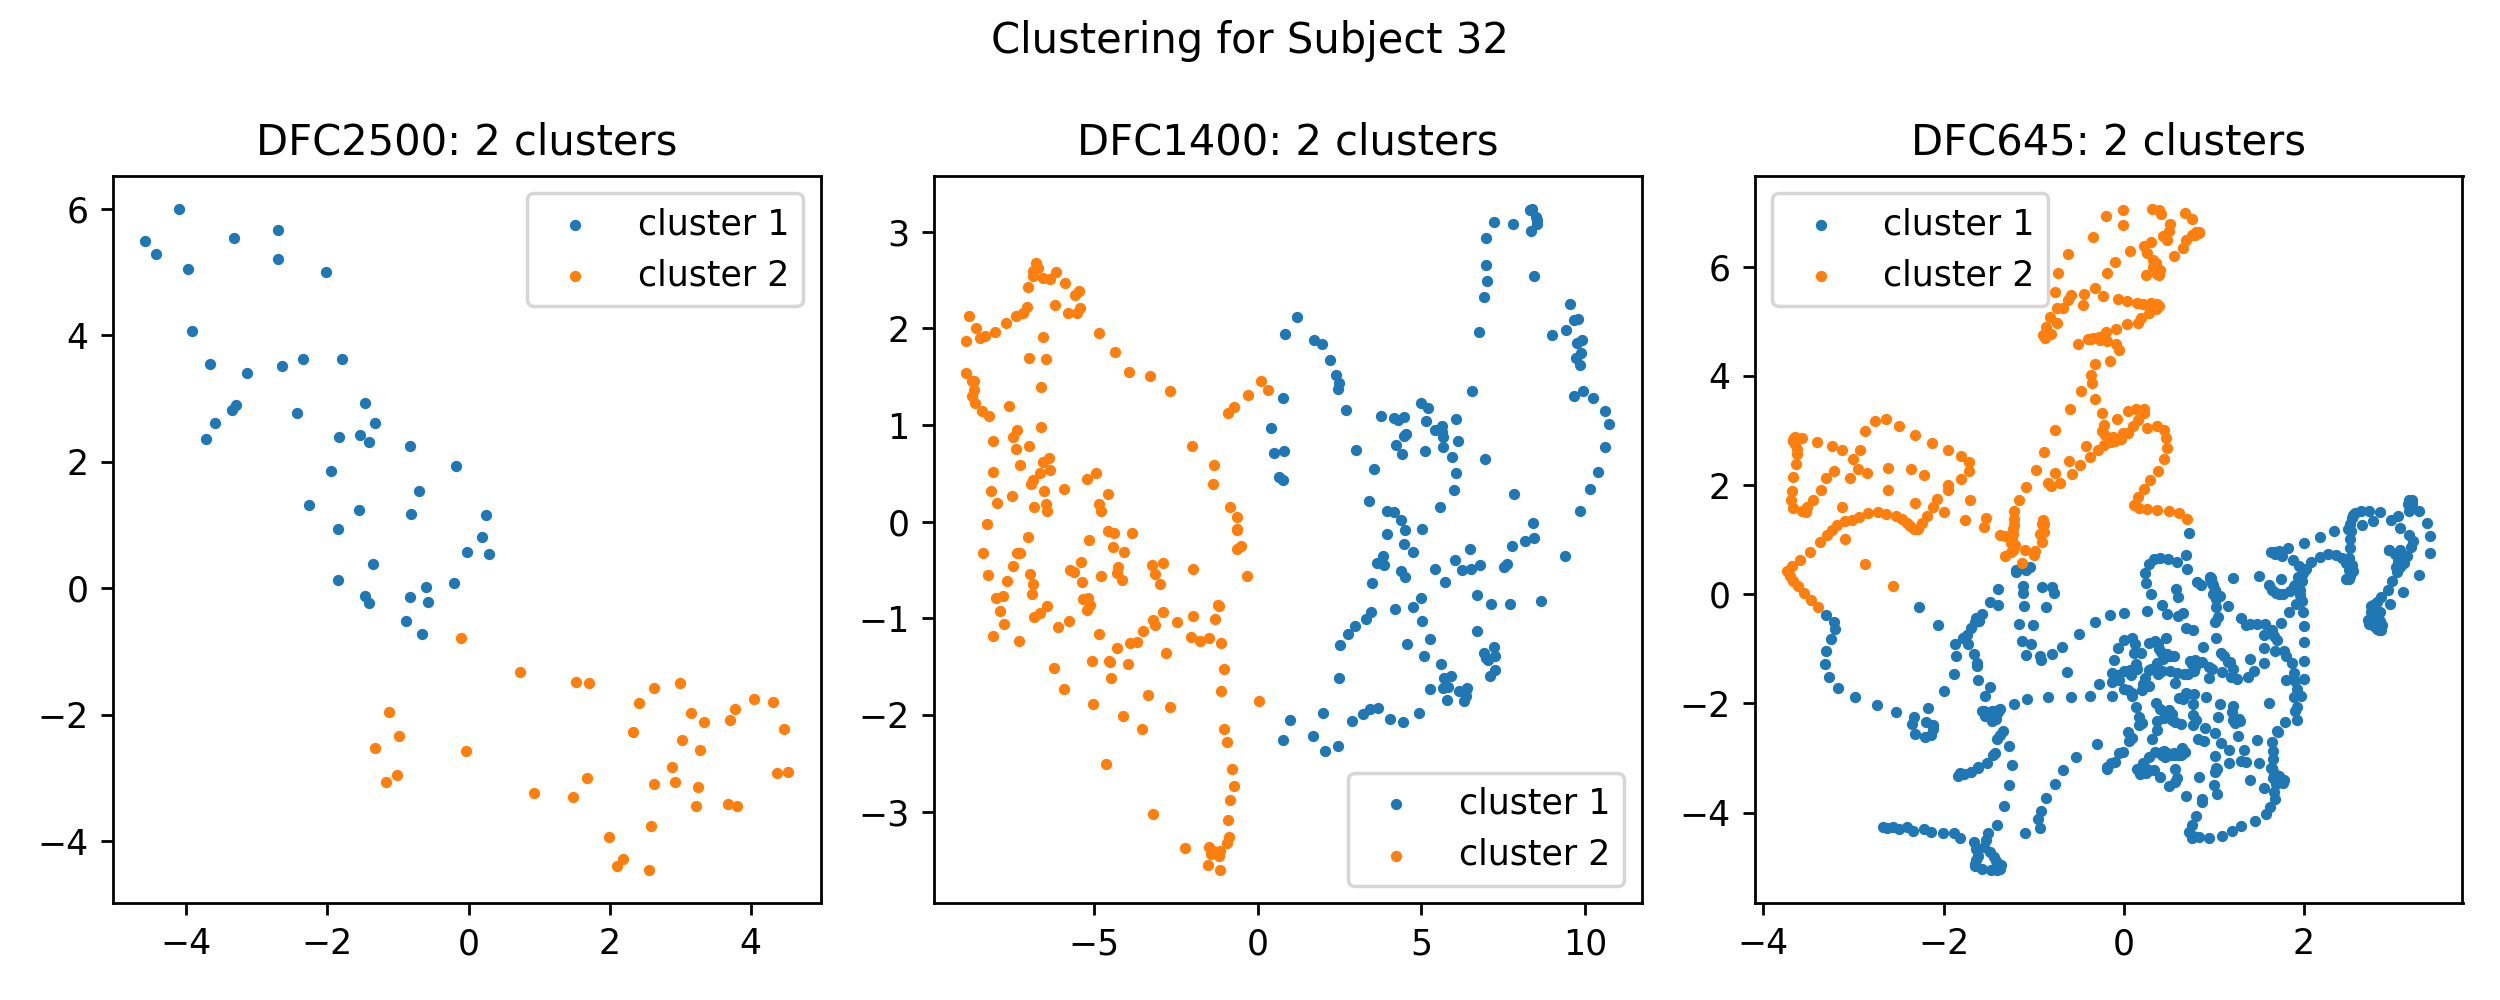
\includegraphics[width=1\textwidth, trim={0cm, 0.0cm, 0.0cm, 0.0cm}]{figures/clusters/subject_32.png}\hfill
	\end{subfigure}
	\begin{subfigure}[!ht]{1\textwidth}
		\centering
		\hspace{8mm}
		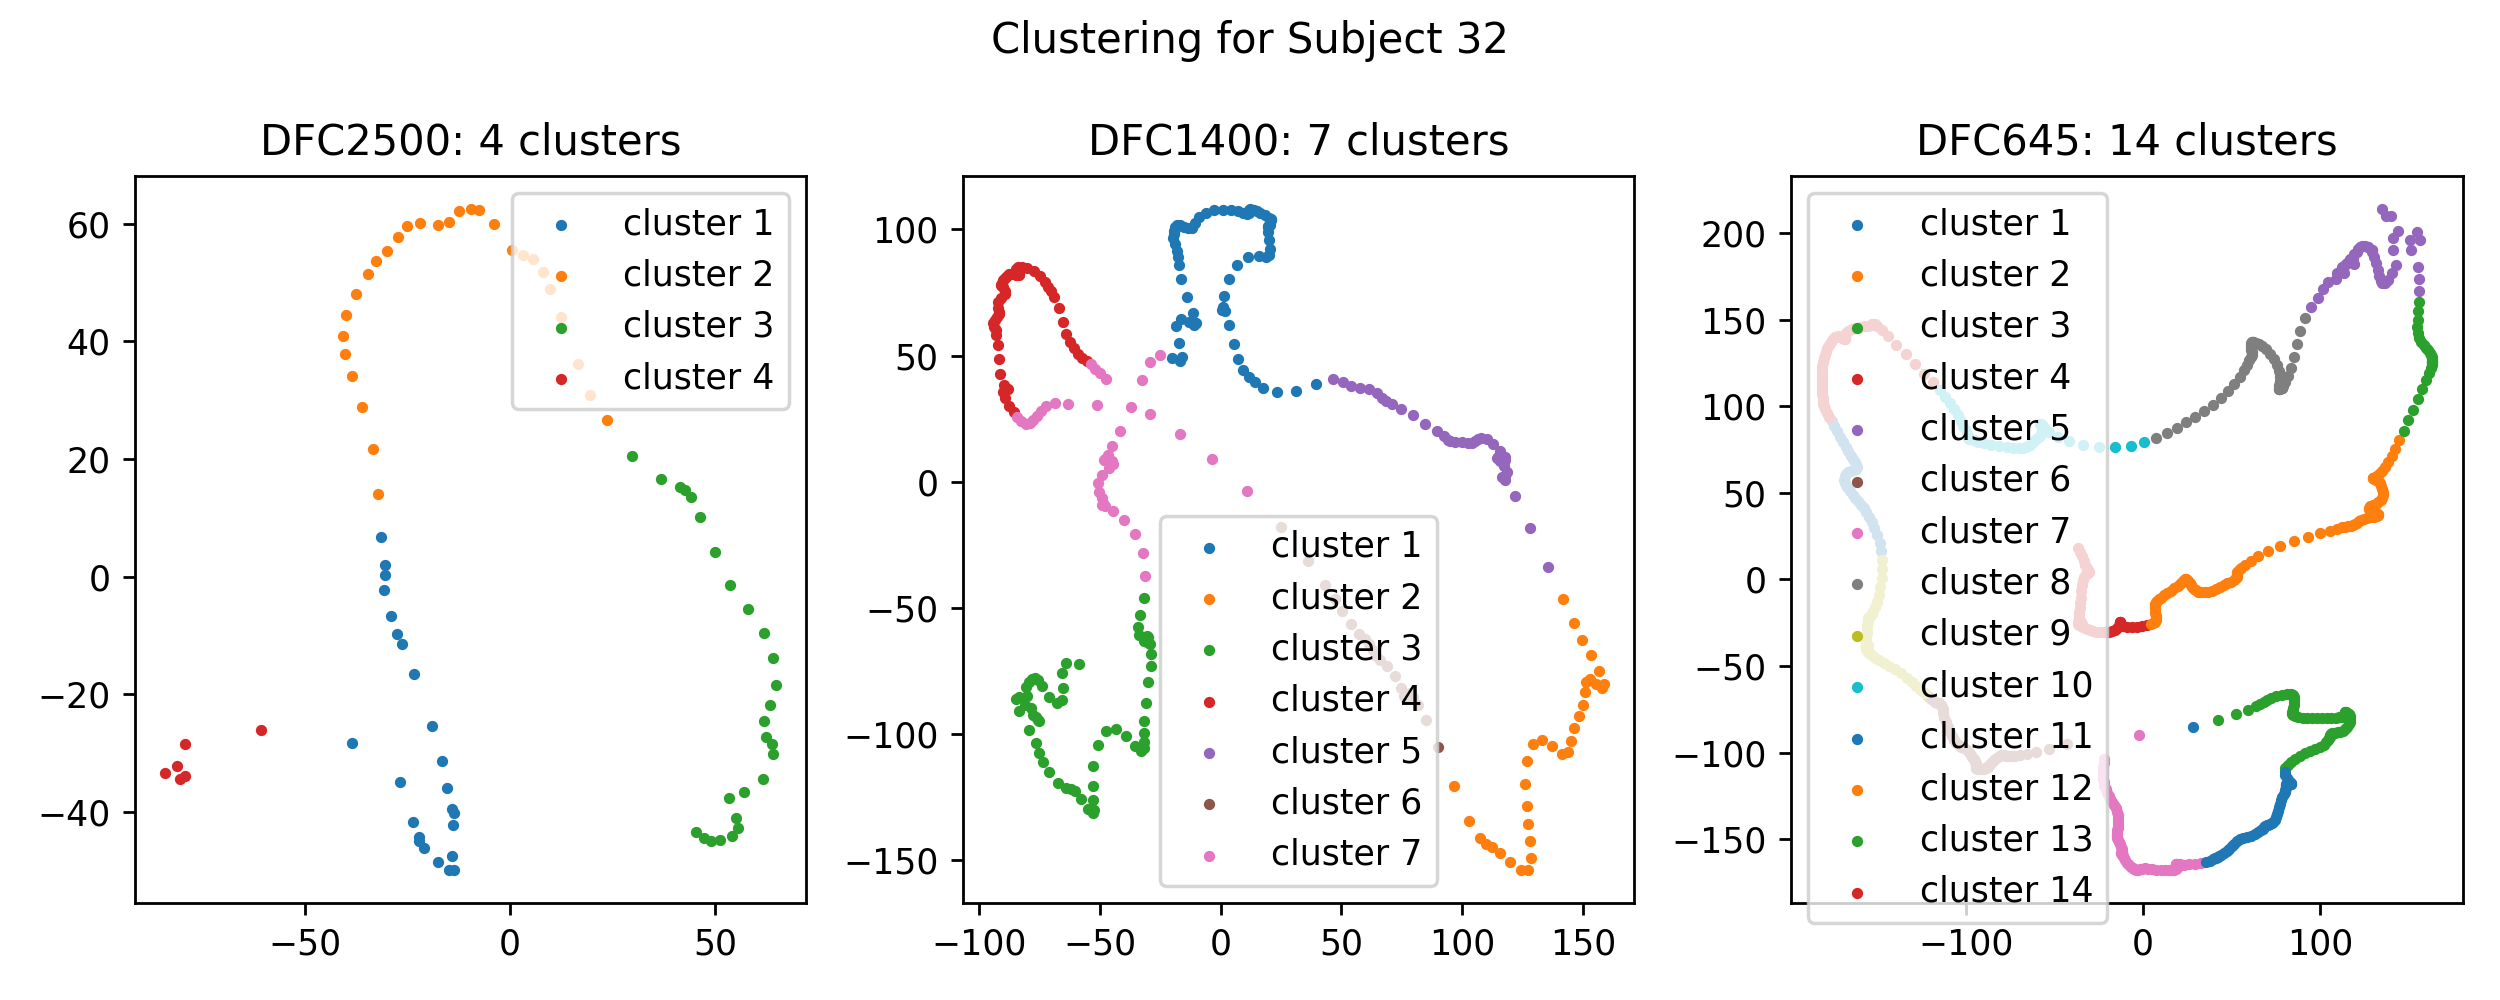
\includegraphics[width=1\textwidth, trim={0cm, 0.0cm, 0.0cm, 0.0cm}]{figures/clusters/subject_32_non_tda.png}\hfill
	\end{subfigure}
	\caption{Clustering result for subject $32$ (top row) for temporal period $2500ms$ (left), $1400ms$ (center), and $645ms$ (right). Clustering result for the same subject (bottom row) with NonTDA Clustering result.}
	\label{fig:clus}
\end{figure}

\section{Results}
\label{sec:eval}
Our TDA and nonTDA pipelines start with embedding one FCN for each rs-fMRI scan as an adjacency matrix (section~\ref{sec:fmri_to_fcn}). In this stage, we get $371,616$ adjacency matrices ($(316 \times 86) + (316 \times 336) + (316 \times 754)$) for three temporal sampling periods ($2500ms$, $1400ms$, $645ms$). Each matrix has a dimension of $113 \times 113$. For example, the FCNs for the three sampling periods for subject $1$ are shown in Figure~\ref{fig:wd1}. In the second stage of the pipelines, we embed the FCN using Pearson's correlation coefficients and range the values between $0$ and $1$. The third stage of the TDA pipeline extracts 0-dimensional persistent barcodes from the matrices using persistent homology (section~\ref{sec:ms_to_pd}). The bottom row of Figure~\ref{fig:wd1} shows the extracted 0-dimensional barcodes for the three TRs. In the nonTDA pipeline, instead of using persistent homology, we used correlation coefficients between the timesteps for the three TRs. We continue to the statistical analysis phase, where we evaluate the resiliency of our TDA framework on different temporal sampling periods of rs-fMRI datasets (section~\ref{sec:si}).


\begin{figure}[!ht]
	\centering
	\begin{subfigure}[!ht]{1\linewidth}
		\centering
		\hspace{8mm}
		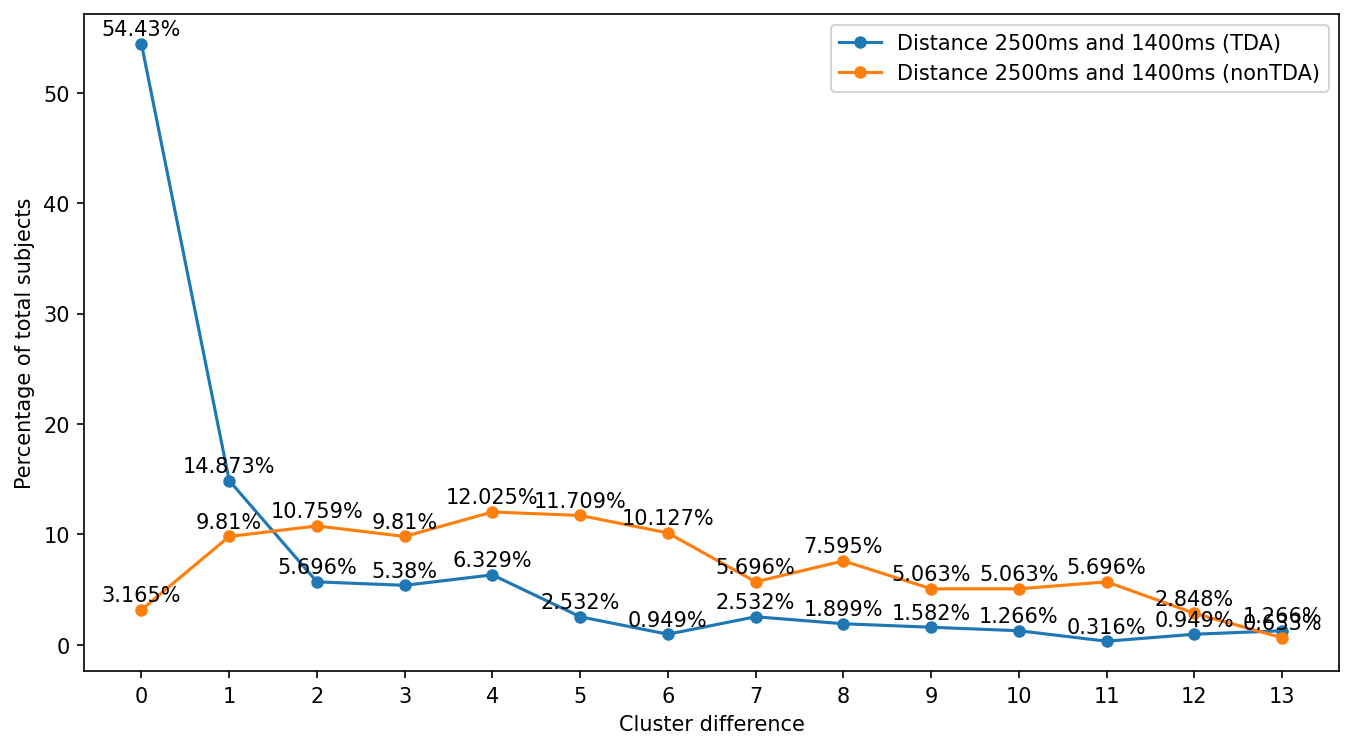
\includegraphics[width=0.8\textwidth, height=0.28\textheight]{figures/pairwise_2500_1400.png}\hfill
		%\hspace{-15mm}
	\end{subfigure}
	\begin{subfigure}[!ht]{1\linewidth}
		\centering
		\hspace{8mm}
		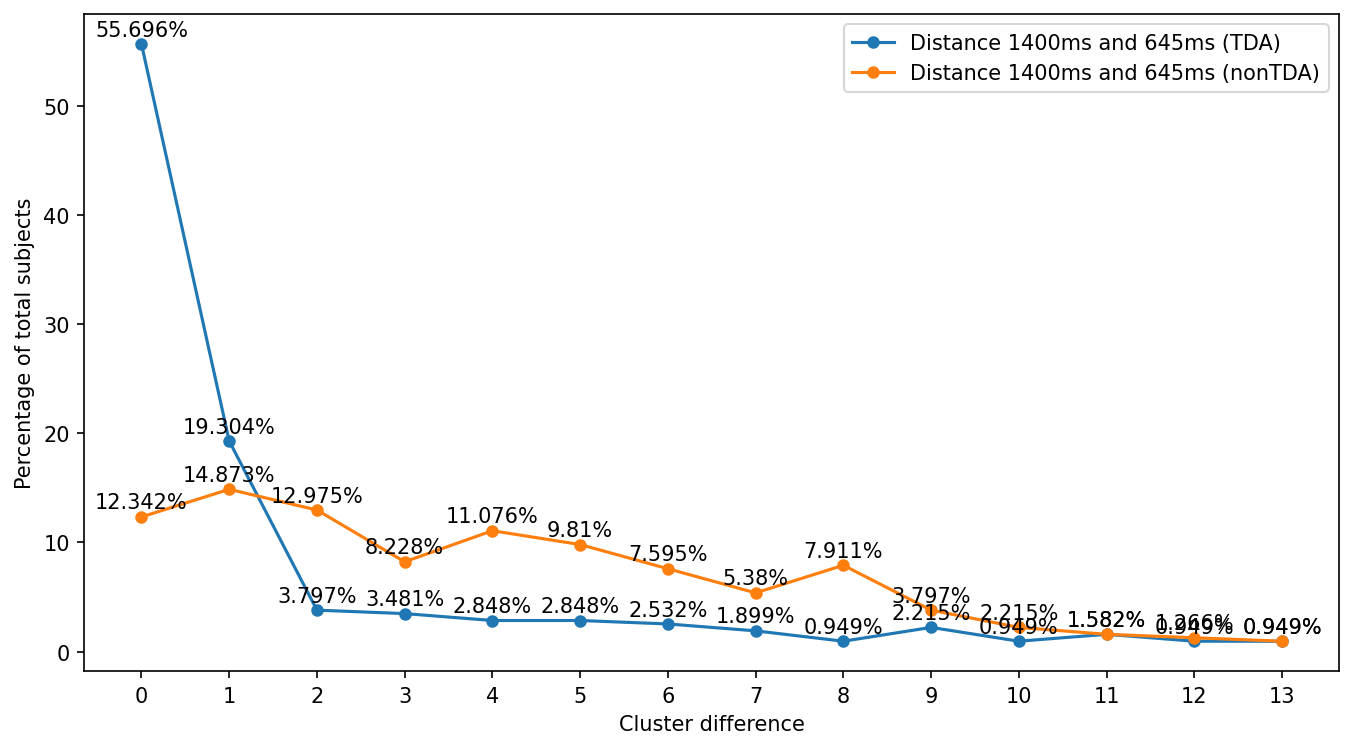
\includegraphics[width=0.8\textwidth, height=0.28\textheight]{figures/pairwise_1400_645.png}\hfill
		%\hspace{-15mm}
	\end{subfigure}
	\begin{subfigure}[!ht]{0.8\linewidth}
		\centering
		\hspace{8mm}
		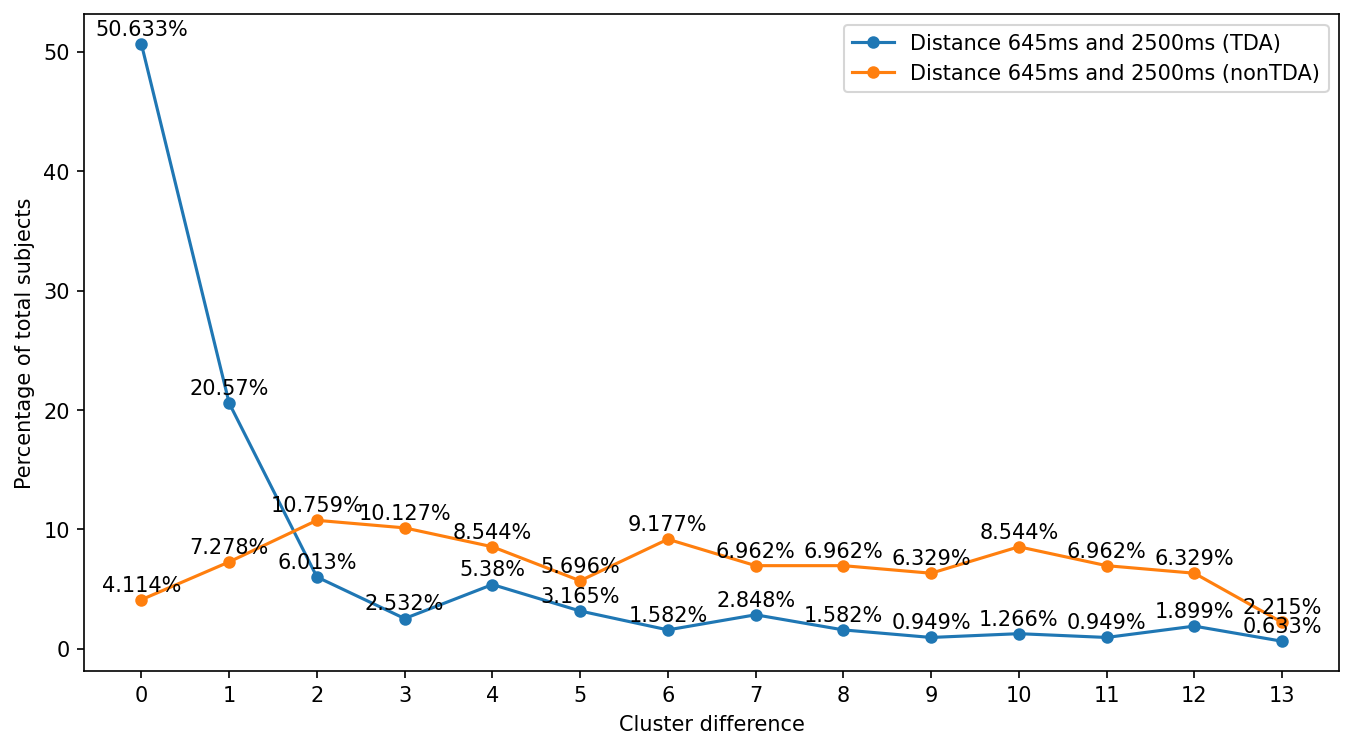
\includegraphics[width=1\textwidth, height=0.28\textheight]{figures/pairwise_645_2500.png}\hfill
		%\hspace{-15mm}
	\end{subfigure}
	\caption{Pairwise cluster distance comparison between TDA and nonTDA pipeline. Comparison between temporal sampling $2500$ and $1400$ (top row), temporal sampling $1400$ and $645$ for TDA and nonTDA pipeline(top row), temporal sampling $645$ and $2500$(bottom row)}
	\label{fig:clus_distance_pairwise}
\end{figure}

In the TDA pipeline, we use the Wasserstein distance metric on the persistent diagrams for all the subjects for all three temporal sampling periods. On the contrary, in the nonTDA pipeline, we directly use the correlation coefficient on the extracted FCNs. Adjacency matrices generated after this stage in both pipelines are similar in size for respective temporal sampling periods. For temporal sampling period $2500ms$ with $86$ timesteps in the TDA pipeline, each subject yields adjacency matrix $WD$ of size ($86 \times 86$) where $WD_{ij}$ represents the pairwise Wasserstein distance between timestep $i$ and $j$. In the nonTDA pipeline for the same data cohort, each subject yields adjacency matrix $A$ of size ($86 \times 86$) where $A_{ij}$ represents the pairwise norm between timestep $i$ and $j$. Similarly, $1400ms$ and $645ms$ yield adjacency matrix of size ($336 \times 336$) and ($754 \times 754$), respectively, for each of the subjects during TDA and nonTDA analysis. This high dimensionality of the matrix size makes it challenging to apply statistical analysis. For this reason, we applied multidimensional scaling (MDS) and reduced the size of the matrices to fit into a two-dimensional surface for all the data cohorts($2500ms$: ($86 \times 2$), $1400ms$: ($336 \times 2$), $645ms$: ($754 \times 2$)). Then, we applied clustering on the MDS data using the k-means clustering algorithm with Sihouette analysis to select the number of clusters. Finally, we get the number of clusters for all 316 subjects for both pipelines. 



Figure \ref{fig:clus} shows the clustering result for a single subject (subject 32) for all three data cohorts ($2500ms$, $1400ms$, $645ms$). The top row of the figure represents the plotted clusters using the TDA pipeline, and we see that each data cohort here has two clusters. The bottom row of the figure shows the plotted clusters for the same subject using the nonTDA pipeline, and the number of clusters varies for the data cohorts. As the number of clusters remains unchanged for different temporal sampling periods using the TDA pipeline and varies largely for the nonTDA pipeline, it shows the invariant of the TDA pipeline. Thus, this illustration gives an intuition towards our hypothesis of the resiliency of persistent homology-based methods to different data acquisition parameters (temporal sampling periods) in brain rs-fMRI data analysis.

\begin{figure}[!ht]%[!htb]
	\centering
	\begin{subfigure}[!ht]{1\textwidth}
		\centering
		\hspace{8mm}
		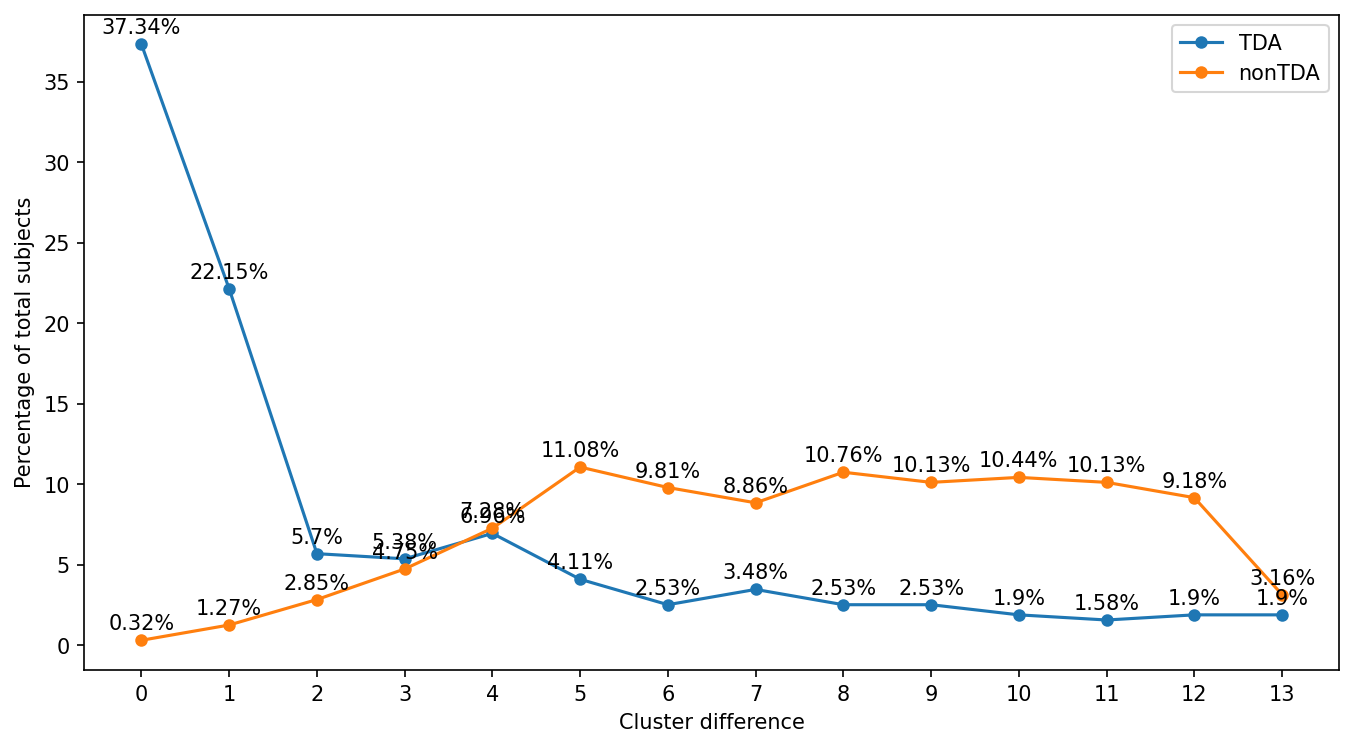
\includegraphics[width=0.8\textwidth]{figures/tda_nontda.png}\hfill
	\end{subfigure}
	\caption{Cluster distance comparison between TDA and nonTDA pipeline}
	\label{fig:clus_distance}
\end{figure}

We capture the number of clusters for 316 subjects for all three data cohorts for both pipelines. We calculate the distance between the number of clusters for each subject using: 

\begin{align}
    distance(subject_i) &= abs(subject_{i_{2500ms}} - subject_{i_{1400ms}})   \nonumber\\
    &+ abs(subject_{i_{1400ms}} - subject_{i_{645ms}})   \nonumber \\ 
    &+ abs(subject_{i_{645ms}} - subject_{i_{2500ms}}) \label{eq:dis}
\end{align}

where $subject_{i_{2500ms}}, subject_{i_{1400ms}}, subject_{i_{645ms}}$ are the number of clusters for $subject_i$ for the data cohorts $2500ms$, $1400ms$, $645ms$ respectively and $abs$ denotes the absolute difference. 
% Table \ref{tab:clustering} 
Figure \ref{fig:clus_distance} shows the distance analysis for both of the pipelines. In the TDA pipeline, we see that majority of the subjects ($59\%$) have a distance less than or equal to one for the data cohorts. On the other hand, in the nonTDA pipeline, less than $2\%$ of the subjects have a distance less than or equal to one. Thus, it shows the resiliency of the persistent homology-based techniques on rs-fMRI data analysis on different data acquisition parameters.




Additionally, we perform a pairwise comparison of the number of clusters for the data cohorts for both of the pipelines. The value of $abs(subject_{i_{2500ms}} - subject_{i_{1400ms}})$ represents the pairwise distance on the number of clusters for $subject_i$ for the data cohorts $2500ms$ and $1400ms$. Similarly, the value of $abs(subject_{i_{1400ms}} - subject_{i_{645ms}})$ and $abs(subject_{i_{645ms}} - subject_{i_{2500ms}})$ represent the pairwise distance on the number of clusters between the data cohorts ($1400ms$, $645ms$) and ($645ms$, $2500ms$) respectively. This pairwise comparison will help to identify whether there is a closer similarity between the data cohorts in the TDA pipeline over the nonTDA pipeline. Figure \ref{fig:clus_distance_pairwise} shows the pairwise distance between the data cohorts in the TDA pipeline. In this pipeline, the pairwise distance between data cohorts $1400ms$ and $645ms$ show the highest similarity ($78\%$ matching within distance 2). The data cohort pair $645ms$ and $2500ms$ has a similarity of $77\%$ within distance two, and data cohort pair $2500ms$ and $1400ms$ has a similarity of $74\%$ within the same distance. This high similarity between the data cohort pairs proves the efficacy of persistent homology-based techniques on the rs-fMRI data analysis with different temporal sampling periods. Table \ref{tab:nontda_between} shows the pairwise distance between the data cohorts in the traditional FCN analysis pipeline (nonTDA). Here, we see the maximum similarity between the data cohorts $1400ms$ and $645ms$ with $40\%$ similarity within distance 2. The other data cohort pairs (($2500ms$, $1400ms$) and ($645ms$, $2500ms$)) has $23\%$ and $22\%$ similarity within the same distance. This low similarity between the data cohorts using traditional FCN analysis indicates the inefficiency of the nonTDA pipeline for analysing rs-fMRI data with different data acquisition parameters. 


Overall, these results demonstrate that TDA captures fundamental temporal properties of rs-fMRI data that are robust to changes in sampling rate. By extracting topological features using persistent homology, TDA provides a more invariant representation of functional brain dynamics compared to traditional functional connectivity methods. This suggests TDA is a promising approach for analyzing complex temporal patterns in resting-state fMRI.




\setlength{\tabcolsep}{0.5em} % for the horizontal padding
{\renewcommand{\arraystretch}{1.2}% for the vertical padding
    \begin{table}[!ht]
        \centering
        \begin{tabular}
        {| c | c | c | c | c | c | c |}
         \hline
            \multirow{2}{*}{Distance} & \multicolumn{2}{c |}{$2500ms$ and $1400ms$ } & \multicolumn{2}{c |}{$1400ms$ and $645ms$ } & \multicolumn{2}{c |}{$645ms$ and $2500ms$ } \\ \cline{2-7}
              & Subjects & Percentage & Subjects & Percentage & Subjects & Percentage
             \\ \hline \hline
0 & 10 & 3.165\% & 39 & 12.342\% & 13 & 4.114\% \\ \hline 
1 & 31 & 9.810\% & 47 & 14.873\% & 23 & 7.278\% \\ \hline 
2 & 34 & 10.759\% & 41 & 12.975\% & 34 & 10.759\% \\ \hline 
3 & 31 & 9.810\% & 26 & 8.228\% & 32 & 10.127\% \\ \hline 
4 & 38 & 12.025\% & 35 & 11.076\% & 27 & 8.544\% \\ \hline 
5 & 37 & 11.709\% & 31 & 9.810\% & 18 & 5.696\% \\ \hline 
6 & 32 & 10.127\% & 24 & 7.595\% & 29 & 9.177\% \\ \hline 
7 & 18 & 5.696\% & 17 & 5.380\% & 22 & 6.962\% \\ \hline 
8 & 24 & 7.595\% & 25 & 7.911\% & 22 & 6.962\% \\ \hline 
9 & 16 & 5.063\% & 12 & 3.797\% & 20 & 6.329\% \\ \hline 
10 & 16 & 5.063\% & 7 & 2.215\% & 27 & 8.544\% \\ \hline 
11 & 18 & 5.696\% & 5 & 1.582\% & 22 & 6.962\% \\ \hline 
12 & 9 & 2.848\% & 4 & 1.266\% & 20 & 6.329\% \\ \hline 
13 & 2 & 0.633\% & 3 & 0.949\% & 7 & 2.215\% \\ \hline
        \end{tabular}
        \caption{Clustering result similarity between cohorts for non TDA pipeline}
        \label{tab:nontda_between}
    \end{table}      



